\chapter{Linear Optics}

%-----------------------------------------------------------------
\section{Coupling and Normal Modes}
\label{s:coupling}
\index{normal mode!Coupling}

The coupling formalism used by \bmad is taken from the paper of Sagan and
Rubin\cite{b:coupling}. The main equations are reproduced here with the notation change that $\bfA$
and $\bfB$ is replaced by $\bfQ$ and $\bfW$\footnote{The reason why $q$ and $w$ are used here to
denote the modes is to avoid confusion with the \bmad convention of using the labels $a$ and $b$ to
represent the same modes throughout the lattice. At the start of the lattice, by convention, the $a$
mode is the same as the $q$ mode and the $b$ mode is the same as the $w$ mode. If there is a ``mode
flip'' (see Sagan and Rubin for an explanation of this term) at some spot in the lattice, the $a$
mode before the mode flip will be the same physical mode after the mode flip (and similarly for the
$b$ mode.  That is, after the mode flip the $a$ mode will be the same as the $w$ mode and the $b$
mode will be the same as the $q$ mode.}

The analysis starts with the map $\bfT(s)$ for the transverse two--dimensional phase space coordinates
$\bfx = (x, x', y, y')$. In ring, with a closed geometry, this map will be a one-turn map starting
and ending at some point $s$. For a machine with open geometry, $\bfT(0)$ can be computed from the
initial Twiss and coupling parameters and $\bfT(s)$ can then be computed by propagating with the
transfer map $\bfM_{0s}$ from $0$ to $s$:
\begin{equation}
    \bfT(s) = \bfM_{0s} \, \bfT(0) \, \bfM_{0s}^{-1}
\end{equation}

$\bfT$ can be decomposed using a similarity transformation
 can be written as
  \begin{equation}
    \bfT = \bfV \, \bfU \, \bfV\inv 
    , \label{tvuv}
  \end{equation} 
where $\bfV$ is symplectic, and $\bfU$ is of the form
  \begin{equation}
    \bfU = 
    \begin{pmatrix}
      \bfQ & \Bf0 \cr 
      \Bf0 & \bfW \cr
    \end{pmatrix}
    . \label{ua00b}
  \end{equation}
\index{normal mode!a--mode}
\index{normal mode!b--mode}
Since $\bfU$ is uncoupled the standard Twiss analysis can be performed on the matrices
$\bfQ$ and $\bfW$. The normal modes are labeled $q$ and $w$ and if the one--turn matrix
$\bfT$ is uncoupled then $w$ corresponds to the horizontal mode and $w$ corresponds to the
vertical mode.

The $\bfQ$ and $\bfW$ matrices can be parameterized using the standard 1-dimensional Twiss
parametrization:
\begin{equation}
  \bfQ = \begin{pmatrix}
    \cos\theta_q + \alpha_q \, \sin\theta_q & \beta_q \, \sin\theta_q \\
    -\gamma_q \, \sin\theta_q & \cos\theta_q - \alpha_q \, \sin\theta_q
    \end{pmatrix}
\end{equation}
and $\bfV$ is written in the form
  \begin{equation}
    \bfV = 
    \begin{pmatrix}
        \gamma \bfI & \bfC \cr 
        -\bfC^+     & \gamma \bfI \cr
    \end{pmatrix}
    , \label{vgicc1}
  \end{equation}
where $\bfC$ is a 2x2 matrix and $+$ superscript 
denotes the symplectic conjugate:
\index{symplectic!conjugate}
  \begin{equation}
    \bfC^+ = 
    \begin{pmatrix}
       C_{22} & -C_{12} \cr 
      -C_{21} & C_{11} \cr
    \end{pmatrix}
    . \label{ccccc}
  \end{equation}
Since we demand that $\bfV$ be symplectic we have the condition
  \begin{equation}               
    \gamma^2 + \, |\bfC| = 1
    , \label{gc1}
  \end{equation}
and $\bfV\inv$ is given by
  \begin{equation}
    \bfV\inv = 
    \begin{pmatrix}
      \gamma \bfI & -\bfC \cr 
      \bfC^+ & \gamma \bfI \cr
    \end{pmatrix}
    . \label{vgicc2}
  \end{equation} 
$\bfC$ is a measure of the coupling. $\bfT$ is uncoupled if and only if $\bfC = \Bf 0$.

It is useful to normalize out the $\beta(s)$ variation in the above analysis. Normalized quantities
being denoted by a bar above them. The normalized normal mode matrix $\BAR\bfU$ is defined by
  \begin{equation}
    \BAR\bfU = \bfG \, \bfU \, \bfG\inv
    , \label{ugug}
  \end{equation}
Where $\bfG$ is given by 
  \begin{equation}
    \bfG \equiv 
    \begin{pmatrix}
      \bfG_q & \Bf0 \cr 
      \Bf0 & \bfG_w
    \end{pmatrix}
    , \label{gg00g}
  \end{equation}  
with 
  \begin{equation}
    \bfG_q = 
    \begin{pmatrix}
      \frac{\tstyle 1}{\tstyle \sqrt{\beta_q}} & 0 \cr
      \frac{\tstyle \alpha_q}{\tstyle \sqrt{\beta_q}} & \sqrt{\beta_q}
    \end{pmatrix}
    , \label{g1b0a} 
  \end{equation}
with a similar equation for $\bfG_w$. With this definition, the corresponding $\BAR\bfQ$ and
$\BAR\bfW$ (cf.~\Eq{ua00b}) are just rotation matrices. The relationship between $\bfT$ and
$\BAR\bfU$ is
  \begin{equation}
    \bfT = \bfG\inv \, \BAR\bfV \, \BAR\bfU \, \BAR\bfV\inv \, \bfG
    , \label{tgvuv}
  \end{equation}
where
  \begin{equation}
    \BAR\bfV = \bfG \, \bfV \, \bfG\inv
    . \label{vgvg}
  \end{equation}
Using \Eq{gg00g}, $\BAR\bfV$ can be written in the form
  \begin{equation}
    \BAR\bfV = 
    \begin{pmatrix}
      \gamma \bfI & \BAR\bfC \cr -\BAR\bfC^+ & \gamma \bfI
    \end{pmatrix}
    , \label{vgicc3}
  \end{equation}
with the normalized matrix $\BAR\bfC$ given by
  \begin{equation}
    \BAR\bfC = \bfG_q \, \bfC \, \bfG_w\inv
    . \label{cgcg}
  \end{equation}

The normal mode coordinates ${\bf q} = (q, q', w, w')$ are related to the laboratory frame via
  \begin{equation}
    {\bf q} = \bfV\inv \, {\bf x}
    . \label{avx}
  \end{equation} 
In particular the normal mode dispersion $\bfeta_q = (\eta_q, \eta'_q, \eta_w, \eta'_w)$ is related
to the laboratory frame dispersion $\bfeta_x = (\eta_x, \eta'_x, \eta_y, \eta'_y)$ via
  \begin{equation}
    {\bfeta_q} = \bfV\inv \, {\bfeta_x}
    . \label{etaavx}
  \end{equation} 
When there is no coupling ($\bfC = 0$), $\bfeta_q$ and $\bfeta_x$ are
equal to each other.

%-----------------------------------------------------------------
\section{Tunes From One-Turn Matrix Eigen Analysis}
\label{s:eigen.tune}

\begin{figure}[tb]
  \centering
  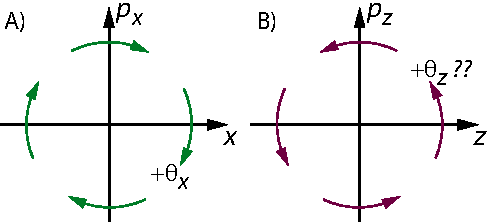
\includegraphics[width=5in]{tune.pdf}
  \caption[Illustration of a positive tune]{A) The standard accelerator physics convention is that 
a clockwise rotation in $(x, p_x)$ or $(y, p_y)$ space represents a positive tune. B) For longitudinal
oscillations, it is sometimes conventional to take counterclockwise rotation as positive if a machine
is always running above transition.}
  \label{f:tune}
\end{figure}

Given the $6 \times 6$ one-turn matrix for a storage ring, one issue is how to extract the tunes. If
there is no coupling the analysis is simple but with coupling things get more complicated. In the
general case, calculating with eigenvectors and eigenvalues gives, assuming that the lattice is
stable, three pairs of eigenvalues with the two eigenvalues of a given pair being complex
conjugates and all eigenvalues having unit amplitude. That is, the eigenvalues $\lambda_i$, $i =
1, \ldots 6$ can be written in the form:
\begin{align}
  \lambda_1, \, \lambda_2 &= \exp(i \, \theta_a), \, \exp(-i \, \theta_a) \CRNO
  \lambda_3, \, \lambda_4 &= \exp(i \, \theta_b), \, \exp(-i \, \theta_b) \label{lleit} \\
  \lambda_5, \, \lambda_6 &= \exp(i \, \theta_c), \, \exp(-i \, \theta_c) \nonumber
\end{align}
where $\theta_a$, $\theta_b$, and $\theta_c$ are the three tunes. To associate $\lambda_1$ and
$\lambda_2$, along with their associated eigenvectors $\bfV_1$ and $\bfV_2$, with the
``horizontal-like'' mode, all the eigenvectors are compared to one another and the eigenvector pair
with the largest values for the $x$ and $p_x$ components are used for $\bfV_1$ and $\bfV_2$.
Similarly, for the ``vertical-like'' mode, eigenvector pair with the largest values for the $y$ and
$p_y$ components are associated with $\bfV_3$ and $bfV_4$, and finally for the ``longitudinal-like''
mode the eigenvector pair with the largest values for the $z$ and $p_z$ components are associated
with $\bfV_5$ and $\bfV_6$.

It can be useful to arrange the eigenvalues such that the odd numbered eigenvalues (1, 3, and 5) are
associated with the tune and and the even numbered eigen values (2, 4, and 6) are associated with
the negative of the tune as arranged in \Eq{lleit}. The algorithm for doing this can be deduced by
first considering the case where the motion is in one-dimension only. Here taken to be $(x, p_x)$ as
shown in \fig{f:tune}. Assuming $\beta_x = 1$ and $\alpha_x = 0$, the one-turn matrix $bfM$ is a
simple rotation matrix
\begin{equation}
  \bfM = \begin{pmatrix}
    \cos(\theta_x) & \sin(\theta_x) \\
   -\sin(\theta_x) & \cos(\theta_x)
  \end{pmatrix}
\end{equation}
where $\theta_x$ is the tune. Notice that, by the standard accelerator physics convention, a
positive tune represents a clockwise rotation. The eignvalues and
eigenvectors are
\begin{alignat}{2}
  \lambda_1 &= \exp( i \, \theta_x),  \qquad &&\bfV_1 = \frac{1}{\sqrt{2}} \, (1, i) \CRNO
  \lambda_2 &= \exp(-i \, \theta_x),  \qquad &&\bfV_2 = \frac{1}{\sqrt{2}} \, (1, -i) 
\end{alignat}
Thus, for the eigenvector $(1, i)/\sqrt{2}$, were the the momentum component is rotated by a factor
of $\pi/2$ counterclockwise from the position coordinate, the rotation angle is the tune. The
rotation angle associated with the eigenvector $(1, -i)/\sqrt{2}$ is associated with the negative of
the tune.

In the general case, each $\bfV_i$, $i = 1, \ldots 6$, is a vector in $(x, p_x, y, p_y, z, p_z)$
space with each component of the vector being a complex number. The criterion that an eigenvector
is associated with the tune is that the phase of the momentum components are on average rotated
clockwise from the position coordinates is
\begin{equation}
  \wt\bfV_{j}^* \, \bfS \, \bfV_j = i, \quad j = 1, 3, 5
  \label{vsvi0}
\end{equation}
where the tilde means transpose and $\bfS$ is the matrix
\begin{equation}
  \bfS = \begin{pmatrix}
      0 & -1 &  0 &  0 &  0 &  0 \\
      1 &  0 &  0 &  0 &  0 &  0 \\
      0 &  0 &  0 & -1 &  0 &  0 \\
      0 &  0 &  1 &  0 &  0 &  0 \\
      0 &  0 &  0 &  0 &  0 & -1 \\
      0 &  0 &  0 &  0 &  1 &  0 \\
  \end{pmatrix}
\end{equation}
\Eq{vsvi0} also makes sure that $\bfV$ is properly normalized.\footnote
  {
Different Authors can use different conventions. For example, the $\bfS$ matrix in the paper by
Ohmi, Hirata, and Oide \cite{b:ohmi}, is the negative of the $\bfS$ matrix defined here and their
phases are reversed (positive phase is counterclockwise rotation) as can be seen from Eqs.~(77) and
(79) in their paper
  }

Note: The longitudinal-like mode is a slight bit tricky here in that, while the mathematics is the
same as for the other modes, in the case where a machine is above transition, what counts as a
positive tune for a User may be a counterclockwise rotation in $(z, p_z)$ space.

%-----------------------------------------------------------------
\section{Dispersion Calculation}
\label{s:dispersion}
\index{dispersion|hyperbf}

The dispersion ($\eta$) and the dispersion derivative ($\eta'$) are defined by the equations
\begin{align}
  \eta_x(s) &\equiv \left. \frac{dx}{dp_z} \right|_s \comma \qquad
    \eta'_x(s) \equiv \left. \frac{d\eta_x}{ds} \right|_s
    = \left. \frac{dx'}{dp_z} \right|_s \CRNO
  \eta_y(s) &\equiv \left. \frac{dy}{dp_z} \right|_s \comma \qquad
    \eta'_y(s) \equiv \left. \frac{d\eta_y}{ds} \right|_s
    = \left. \frac{dy'}{dp_z} \right|_s \\
  \eta_z(s) &\equiv \left. \frac{dz}{dp_z} \right|_s \nonumber
\end{align}

Given the dispersion at a given point, the dispersion at some other point is calculated as follows:
Let $\Bf r = (x, p_x, y, p_y, z, p_z)$ be the reference orbit, around which the dispersion is to be
calculated. Let $\bfV$ and $\bf M$ be the zeroth and first order components of the transfer map
between two points labeled 1 and 2:
\begin{equation}
  \Bf r_2 = \bfM \, \Bf r_1 + \bfV
  \label{rmrv}
\end{equation}
Define the dispersion vector $\bfeta$ by
\begin{equation}
  \bfeta = 
  \left( 
    \eta_x, \eta'_x \, (1 + p_z), \eta_y, \eta'_y \, (1 + p_z), \eta_z, 1
  \right)
\end{equation}
Differentiating \Eq{rmrv} with respect to energy, the dispersion at point 2 in terms of the
dispersion at point 1 is
\begin{equation}
  \bfeta_2 = \left[ \frac{dp_{z2}}{dp_{z1}} \right]^{-1} \, 
    \left[ \bfM \, \bfeta_1 \right] + \bfV_\eta 
    \label{eppmev}
\end{equation}
where
\begin{equation}
  \bfV_\eta = \left[ \frac{dp_{z2}}{dp_{z1}} \right]^{-1} \, 
  \frac{1}{1 + p_{z1}}
  \left(
  \begin{array}{c}
    M_{12} \, p_{x1} + M_{14} \, p_{y1} \\
    M_{22} \, p_{x1} + M_{24} \, p_{y1} \\
    M_{32} \, p_{x1} + M_{34} \, p_{y1} \\
    M_{42} \, p_{x1} + M_{44} \, p_{y1} \\
    M_{52} \, p_{x1} + M_{54} \, p_{y1} \\
    M_{62} \, p_{x1} + M_{64} \, p_{y1} \\
  \end{array}
  \right)
  -
  \left(
  \begin{array}{c}
    0 \\
    \frac{p_{x2}}{1 + p_{z2}} \\
    0 \\
    \frac{p_{y2}}{1 + p_{z2}} \\
    0 \\
    0 
  \end{array}
  \right)
\end{equation}
The sixth row of the matrix equation gives $dp_{z1}/dp_{z2}$. 
Explicitly
\begin{equation}
  \frac{dp_{z2}}{dp_{z1}} =
  \sum_{i=1}^6 M_{6i} \, \eta_{1i} + 
  \frac{M_{62} \, p_{x1} + M_{64} \, p_{y1}}{1 + p_{z1}}
\end{equation}
For everything except \vn{RFcavity} and \vn{Lcavity} elements, 
$dp_{z2}/dp_{z1}$ is 1.

For a non-circular machine, there are two ways one can imagine defining the dispersion: Either with
respect to changes in energy at the beginning of the machine or with respect to the local change in
energy at the point of measurement. The former definition will be called ``non-local dispersion''
and the latter definition will be called ``local dispersion''. For a circular machine, local
dispersion is always used.  The dispersion defined in the above equations, which is what \bmad uses
in calculations, is the local dispersion. The non-local dispersion $\wt\bfeta(s_1)$ at some point
$s_1$ is related to the local dispersion $\bfeta(s_1)$ via
\begin{equation}
  \wt\bfeta(s_1) = \frac{dp_{z1}}{dp_{z0}} \, \bfeta(s_1)
\end{equation}
where $s_0$ is the beginning of the machine.

For a non-circular machine, there are advantages and disadvantages to using either local or
non-local dispersion. Local dispersion has the problem that $dp_{z2}/dp_{z1}$ in \Eq{eppmev} may go
through zero at a point producing infinite dispersions at that point. The non-local dispersion has
the merit of reflecting what one would measure if the starting energy of the beam is varied. The
local dispersion, on the other hand, reflects the correlations between the particle energy and
particle position within a beam.

